\documentclass{article}
\usepackage[polish]{babel}
\usepackage[T1]{fontenc}
\usepackage[utf8]{inputenc}
\usepackage{graphicx}
\usepackage{float}
\usepackage[bottom=1.5cm, right=2.5cm, left=2.5cm, top=1.5cm]{geometry}
\graphicspath{{../pliki}}



\title{%
  Cyberbezpieczeństwo - laboratoria 11 \\
  \large Rekonnesans sieciowy}
\author{Patryk Łuszczek 272707}
\date{\today}
\begin{document}
\maketitle
\newpage

Adresy IP maszyn wirtualnych:
\begin{itemize}
  \item Kali: 10.0.4.4
  \item Ubuntu: 10.0.4.6
  \item Metasploitable: 10.0.4.7
  \item Sieć: 10.0.4.0
\end{itemize}

\section*{Badanie sieci za pomocą polecenia nmap}
\begin{figure}[H]
  \centering
  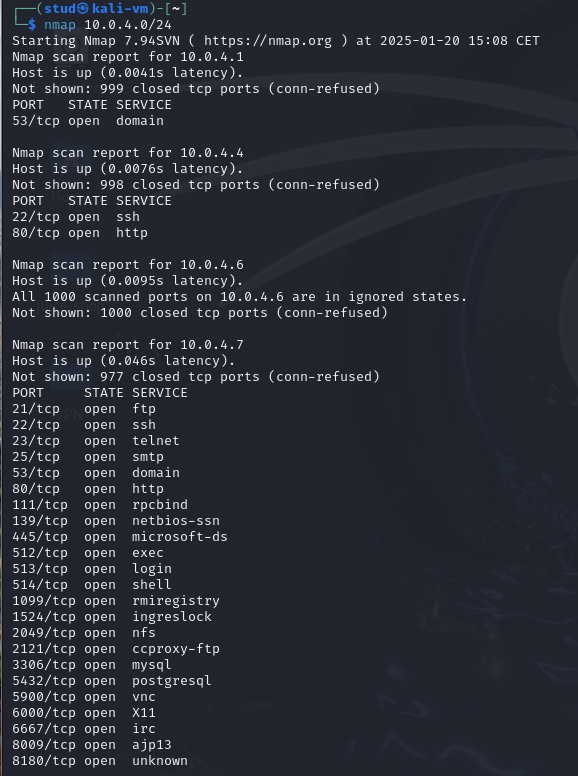
\includegraphics[width=0.7\textwidth]{nmap_siec.png}
  \caption{Skanowanie sieci}
\end{figure}
Odnaleziono 3 hostów w sieci, są to trzy maszyny wirtualne z adresami opisanymi wcześniej.
Można zauważyć otwarte porty na każdym urządzeniu. Kali ma 2 otwarte porty (ssh, http), ubuntu ma wszystkie zamknięte, a metasploitable ma najwięcej
otwartych portów - 23 (np. mysql, postgres).

\section*{Badanie sieci z wykorzystaniem różnych rodzajów skanowania nmap}

\subsection*{Skanowanie w trybie TCP Connect (-sT)}
Tryb -sT nawiązuje pełne połączenie TCP za pomocą \texttt{connect()}, co czyni go powolnym i łatwym do wykrycia. Metoda ta jest używana domyślnie bez uprawnień roota, ale nie ujawnia adresu MAC hosta docelowego.

\begin{figure}[H]
  \centering
  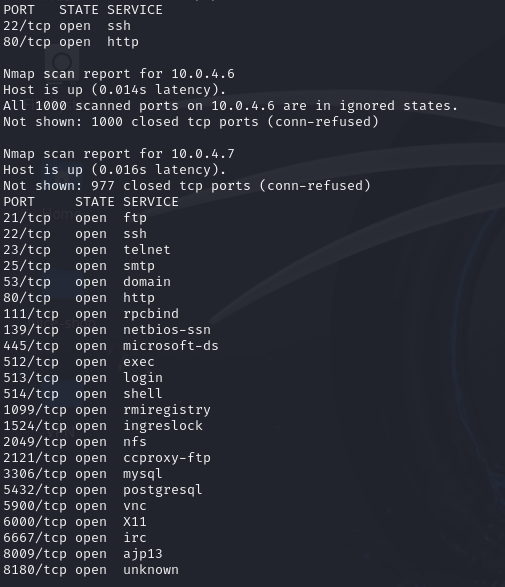
\includegraphics[width=0.7\textwidth]{nmap_st.png}
  \caption{nmap -sT}
\end{figure}

\subsection*{Skanowanie w trybie SYN (-sS)}
Tryb -sS wysyła tylko pakiety SYN i nie nawiązuje pełnego połączenia, co czyni go szybszym i trudniejszym do wykrycia. Odpowiedzi SYN/ACK oznaczają otwarte porty, RST zamknięte, a brak odpowiedzi wskazuje porty filtrowane.

\begin{figure}[H]
  \centering
  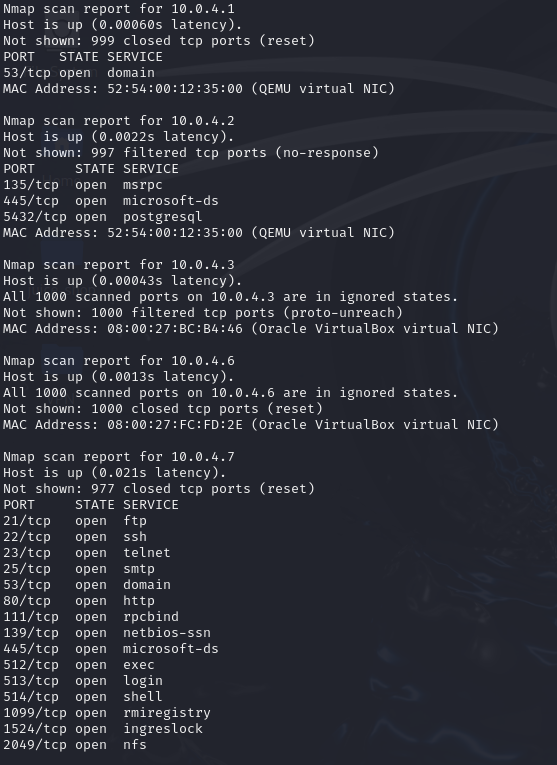
\includegraphics[width=0.7\textwidth]{nmap_ss.png}
  \caption{nmap -sS}
\end{figure}

\subsection*{Skanowanie bez flag (-sN), FIN (-sF) i Xmas (-sX)}
Tryby -sN, -sF i -sX różnią się ustawieniem flag TCP (brak flag, FIN lub FIN, PSH i URG). Pozwalają one wykrywać porty otwarte|filtrowane na podstawie standardu RFC793, ale mogą nie działać na systemach niestandardowych.

\begin{figure}[H]
  \centering
  \includegraphics[width=0.7\textwidth]{nmap_sN.png}
  \caption{nmap -sN}
\end{figure}

\subsection*{Skanowanie w trybie Maimon (-sM)}
Tryb -sM używa pakietów z flagami FIN/ACK, oczekując odpowiedzi RST. Metoda ta działa na systemach niestandardowo implementujących TCP, gdzie wszystkie porty mogą być oznaczane jako zamknięte.

\begin{figure}[H]
  \centering
  \includegraphics[width=0.7\textwidth]{nmap_sM.png}
  \caption{nmap -sM}
\end{figure}

\subsection*{Skanowanie w trybie ACK (-sA)}
Tryb -sA wysyła pakiety ACK, aby sprawdzić filtrowanie stanowe i identyfikować porty filtrowane. Porty otwarte i zamknięte odpowiadają pakietem RST, podczas gdy brak odpowiedzi oznacza filtrowanie.

\begin{figure}[H]
  \centering
  \includegraphics[width=0.7\textwidth]{nmap_sA.png}
  \caption{nmap -sA}
\end{figure}

\subsection*{Skanowanie w trybie Window (-sW)}
Tryb -sW analizuje pole rozmiaru okna w pakietach RST, aby rozróżniać porty otwarte od zamkniętych. Skuteczność metody zależy od implementacji stosu TCP w systemie docelowym.

\begin{figure}[H]
  \centering
  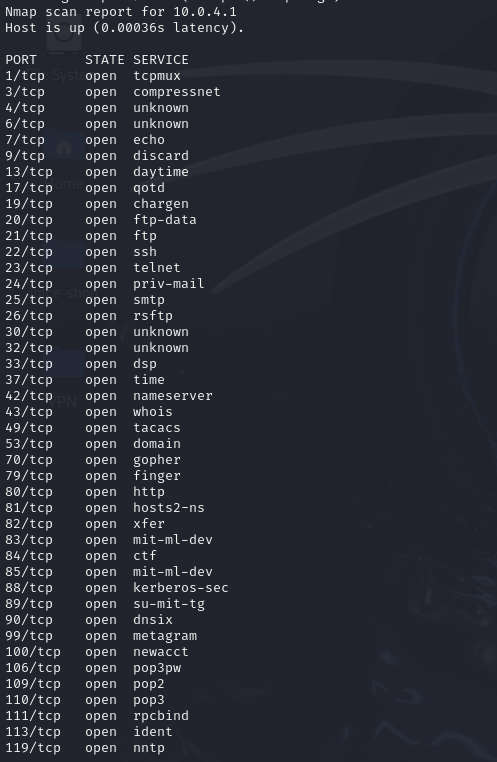
\includegraphics[width=0.7\textwidth]{nmap_sW.png}
  \caption{nmap -sW}
\end{figure}

\subsection*{Skanowanie w trybie UDP (-sU)}
Skanowanie UDP polega na wysyłaniu pustych pakietów UDP do portów docelowych i analizie odpowiedzi. Brak odpowiedzi oznacza port otwarty|filtrowany, odpowiedź ICMP port unreachable wskazuje port zamknięty, a pakiet UDP potwierdza, że port jest otwarty. Metoda ta jest czasochłonna, ponieważ otwarte lub filtrowane porty często nie wysyłają odpowiedzi, co wymusza powtórzenia transmisji.

\section*{Skanowanie z wykorzystaniem opóźnienia (-T)}
Opcja -T pozwala na określenie poziomu intensywności skanowania, co wpływa na jego szybkość i wykrywalność. Nmap oferuje sześć predefiniowanych poziomów:

\begin{itemize}
  \item \textbf{-T0 (Paranoid)}: Skierowane do skanowania w sieciach silnie monitorowanych, generuje bardzo długie opóźnienia między wysyłanymi pakietami.
  \item \textbf{-T1 (Sneaky)}: Powolne skanowanie z mniejszym opóźnieniem niż -T0, wciąż trudne do wykrycia.
  \item \textbf{-T2 (Polite)}: Zmniejsza obciążenie sieci, dodając umiarkowane opóźnienia, aby uniknąć zakłóceń.
  \item \textbf{-T3 (Normal)}: Domyślny poziom intensywności, który zapewnia równowagę między szybkością a dyskrecją.
  \item \textbf{-T4 (Aggressive)}: Zoptymalizowane pod kątem szybkości, odpowiednie dla niezabezpieczonych lub testowych środowisk.
  \item \textbf{-T5 (Insane)}: Bardzo szybkie skanowanie, wymagające stabilnego łącza i sieci o niskim opóźnieniu, ale łatwe do wykrycia.
\end{itemize}

\section*{Skanowanie w celu identyfikacji wersji serwisu na porcie (-sV ... -p)}

\begin{figure}[H]
  \centering
  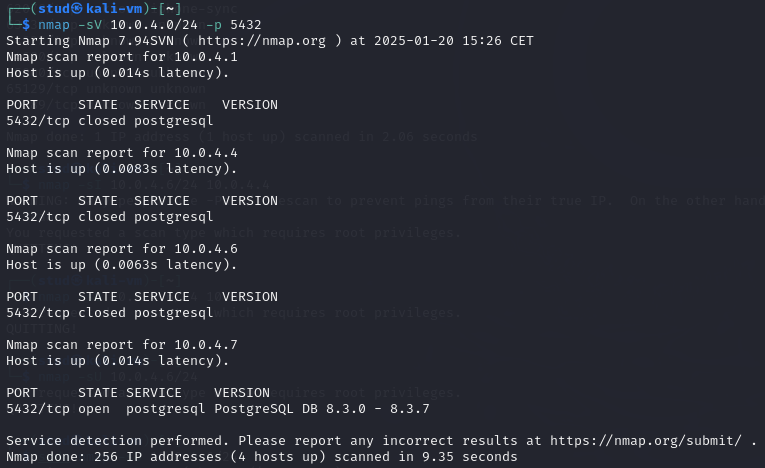
\includegraphics[width=0.7\textwidth]{nmap_port_wersja.png}
  \caption{nmap -sV, -p}
\end{figure}

Za pomocą komendy -sV w połączeniu z numerem portu możemy wykryć wersję usługi uruchomionej na wybranym porcie. Pozwala to na wykrycie potencjalnych luk w zabezpieczeniach, które mogą znacząco ułatwić atak.

\section*{Skanowanie w celu identyfikacji systemu operacyjnego urządzenia}

\begin{figure}[H]
  \centering
  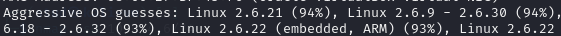
\includegraphics[width=0.6\textwidth]{nmap_os_matplot.png}
  \caption{nmap -O}
\end{figure}

Za pomocą flagi -O możemy wykryć system operacyjny urządzenia. Dla naszych maszyn wirtualnych narzędzie nmap było w stanie wykryć prawdopobny system maszyny z Matsploitable jednak nie z 100\% pewnością.

\section*{Skanowanie z użyciem skryptów}

\begin{figure}[H]
  \centering
  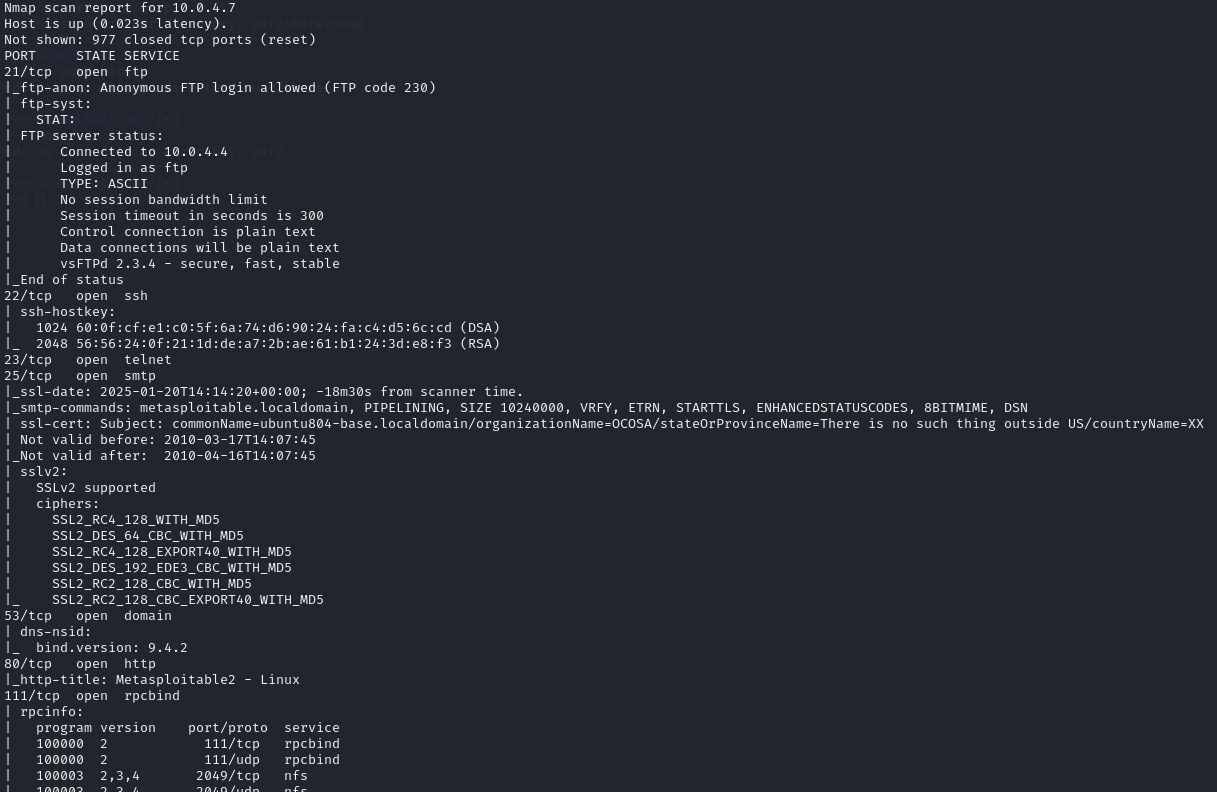
\includegraphics[width=0.7\textwidth]{nmap_sc.png}
  \caption{nmap -sC, domyślne skrypty}
\end{figure}

\begin{figure}[H]
  \centering
  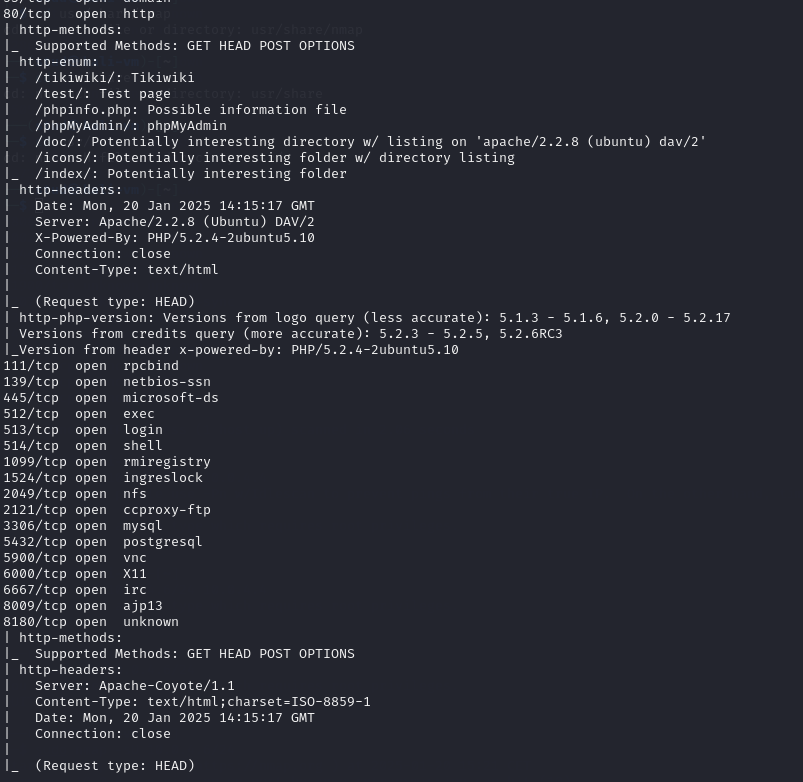
\includegraphics[width=0.7\textwidth]{http_meta_headers.png}
  \caption{nmap z wykorzystaniem wybranych skryptów}
\end{figure}

\begin{itemize}
  \item \textbf{http-enum.nse} – identyfikuje katalogi używane przez popularne aplikacje i serwery webowe na hoście docelowym, co może pomóc w wykryciu podatności,
  \item \textbf{http-headers.nse} – wykonuje żądanie HEAD na katalogu głównym serwera i wyświetla zwrócone nagłówki HTTP, dostarczając informacje o serwerze, jego konfiguracji i obsługiwanym kodowaniu,
  \item \textbf{http-methods.nse} – wysyła żądanie OPTIONS, wskazując obsługiwane przez serwer HTTP metody, oraz identyfikuje potencjalnie niebezpieczne opcje inne niż GET, HEAD, POST i OPTIONS,
  \item \textbf{http-php-version.nse} – podejmuje próbę uzyskania informacji o wersji PHP na serwerze webowym działającym na hoście.
\end{itemize}


\section*{Mapowanie topologi sieci za pomocą Zenmap}

\begin{figure}[H]
  \centering
  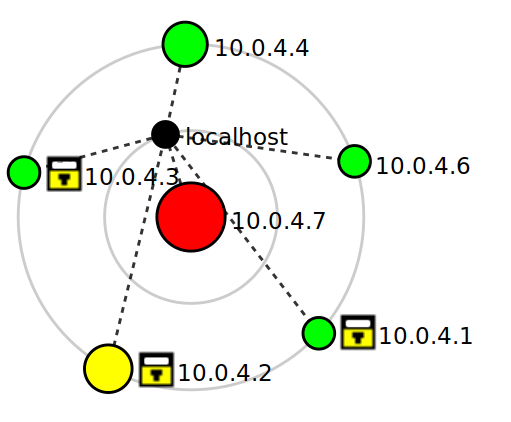
\includegraphics[width=0.7\textwidth]{zenmap_topology.png}
  \caption{Struktura sieci}
\end{figure}



\begin{figure}[H]
  \centering
  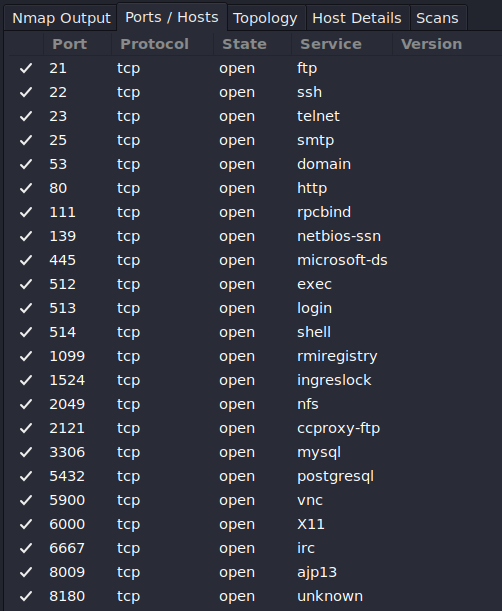
\includegraphics[width=0.7\textwidth]{zenmap_services.png}
  \caption{Odkryte serwisy}
\end{figure}

\begin{figure}[H]
  \centering
  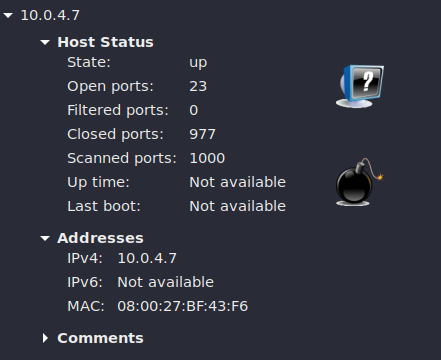
\includegraphics[width=0.7\textwidth]{zenmap_meta.png}
  \caption{Informacje dot. metasplotable}
\end{figure}

\begin{figure}[H]
  \centering
  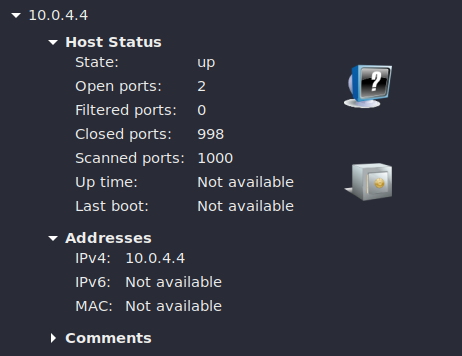
\includegraphics[width=0.7\textwidth]{zenmap_ubuntu.png}
  \caption{Informacje dot. ubuntu}
\end{figure}

Zenmap umożliwia korzystanie z poleceń nmap w bardziej przystępnej formie dzięki graficznej wizualizacji sieci. Wyniki skanowania są takie same jak w nmap, ale prezentowane w sposób wizualny, co pozwoliło na wykrycie wszystkich hostów w sieci, w tym tych uruchomionych przez VirtualBox, jak brama domyślna (10.0.4.1) czy serwer DHCP (10.0.4.2).
\section*{Skanowanie za pomocą amap}
Niestety mimo wielu prób, aktualizacji i zmian konfiguracji nie udało się uruchomić narzędzia amap.
Amap służy do identyfikacji serwisu uruchomionego na danym porcie, a następnie jest ona porównywana z typowym portem działającym na tym porcie. Ponieważ, serwis może być uruchomiony na innym porcie niż domyślny, narzędzie
pozwala na odnalezienie jaka usługa jest faktycznie uruchomiona na tym porcie.

\section*{Pytania}

\begin{enumerate}
  \item \textbf{Czy wyniki uzyskane przez nmap są wiarygodne?} \\
        Wyniki nmap są wiarygodne, ale zależą od konfiguracji systemu i zabezpieczeń hosta oraz sieci. Zastosowany firewall może sprawić, że niektóre porty zostaną uznane za zamknięte, mimo że są otwarte, a usługi na portach mogą różnić się od wskazanych przez nmap, który opiera się na standardowych przypisaniach portów.

  \item \textbf{Czy uzyskane informacje o hoście docelowym zależą od opcji skanowania?} \\
        Opcje skanowania wpływają na szczegółowość i dokładność wyników. Skanowanie z uprawnieniami roota dostarcza więcej danych, takich jak wersje usług czy system operacyjny, podczas gdy różne flagi TCP i protokoły (np. UDP) pozwalają na różnorodną analizę w zależności od konfiguracji hosta.

  \item \textbf{Czy można używać nmap do skanowania hostów bez pozwolenia?} \\
        Nmap jest narzędziem legalnym, jednak skanowanie bez pozwolenia może być uznane za niezgodne z prawem w wielu krajach. Takie działanie może być traktowane jako włamanie do sieci, co wiąże się z odpowiedzialnością karną zgodnie z przepisami dotyczącymi bezpieczeństwa.
\end{enumerate}





\end{document}